% GNN-AoI: Final Project Presentation (LaTeX Beamer, Madrid theme)
% Compile:  tectonic main.tex      (or on Overleaf: pdfLaTeX or XeLaTeX)
\documentclass[aspectratio=169,10pt]{beamer}
\usepackage[utf8]{inputenc}

\usetheme{Madrid}
\usecolortheme{default}

\usepackage{amsmath,amssymb,bm}
\usepackage{booktabs,tabularx,array,multirow,makecell}
\usepackage{graphicx}
\usepackage{tikz}
\usetikzlibrary{arrows.meta,positioning,shapes.geometric,fit,calc,backgrounds,shadows}
\usepackage{algorithm}
\usepackage{algpseudocode}
\usepackage{xcolor}
\usepackage{fontawesome5}

% colours used in figures, diagrams and highlights
\definecolor{ink}{HTML}{0F172A}
\definecolor{inksoft}{HTML}{334155}
\definecolor{muted}{HTML}{64748B}
\definecolor{accent}{HTML}{2563EB}
\definecolor{accentlight}{HTML}{DBEAFE}
\definecolor{good}{HTML}{059669}
\definecolor{bad}{HTML}{DC2626}
\definecolor{orangeb}{HTML}{EA580C}
\definecolor{paper}{HTML}{F8FAFC}
\definecolor{rule}{HTML}{E2E8F0}

\setbeamertemplate{navigation symbols}{}
\newcommand{\hl}[1]{{\color{accent}\textbf{#1}}}
\newcommand{\good}[1]{{\color{good}\textbf{#1}}}
\newcommand{\bad}[1]{{\color{bad}\textbf{#1}}}
\renewcommand{\cite}[1]{{\color{muted}[#1]}}
\newcommand{\sect}[1]{\par{\color{muted}\scriptsize\MakeUppercase{#1}}\par\vspace{0.2em}}
\newcolumntype{Y}{>{\raggedright\arraybackslash}X}
\renewcommand{\arraystretch}{1.15}

\tikzset{
  box/.style={draw=#1,fill=#1!8,rounded corners=4pt,align=center,inner sep=5pt,font=\small},
  box/.default=accent,
  arr/.style={-{Stealth[length=2.2mm]},thick,color=inksoft},
  lab/.style={font=\scriptsize,color=muted,align=center},
  st/.style={box=#1,minimum height=1.25cm,text width=2.25cm,font=\scriptsize},
}

%------------------------------------------------------------
%This block of code defines the information to appear in the
%Title page
\title[GNN-AoI] %optional
{GNN-AoI: Correlation-Aware Scheduling of Real Sensor Networks}

\subtitle{A graph neural network, trained with reinforcement learning, that decides which sensors may transmit under a hard Age-of-Information guarantee}

\author[Palella, Gullanki, Preethikha, Madhumitha] % (optional)
{Bhanu Prasad Palella \and Gullanki Bhagya Lakshmi \and Pavna Preethikha \and Madhumitha S}

\institute[ASAI] % (optional)
{
  Amrita School of Artificial Intelligence\\[0.3em]
  Guide: [guide's name and designation]
}

\date[Final Review] % (optional)
{Final Project Presentation, [presentation date]}

%\logo{\includegraphics[height=1cm]{logo}}   % add a college logo file here if needed

%End of title page configuration block
%------------------------------------------------------------

\begin{document}

%The next statement creates the title page.
\frame{\titlepage}

%---------------------------------------------------------
%Table of contents after the title page
\begin{frame}
\frametitle{Table of Contents}
\tableofcontents
\end{frame}
%---------------------------------------------------------

\section{Introduction}

% =================================================================== 2 PROBLEM
\begin{frame}{Problem Statement}
  \begin{columns}[T]
    \begin{column}{0.56\textwidth}
      \begin{itemize}\setlength\itemsep{0.45em}
        \item A sink must track the readings of \hl{$M$ sensors} (temperature, traffic speed, \dots)
              over a shared wireless channel.
        \item Only \hl{$C \ll M$ sensors may transmit per slot}: the sink must choose \emph{which}.
        \item Classic schedulers minimise the \hl{Age of Information} (AoI) and poll whoever is stalest,
              ignoring \emph{content}: correlated neighbours are polled as if independent.
        \item This wastes capacity on \textbf{redundant data} and worsens the sink's estimate of the field.
      \end{itemize}
      \vspace{0.2em}

    \end{column}
    \begin{column}{0.42\textwidth}
      \centering
      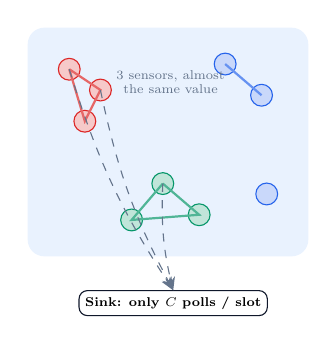
\begin{tikzpicture}[scale=0.66,every node/.style={transform shape}]
        \fill[accentlight!60,rounded corners=6pt] (-0.2,-0.2) rectangle (5.2,4.2);
        \foreach \x/\y/\c in {0.6/3.4/bad,1.2/3.0/bad,0.9/2.4/bad,3.6/3.5/accent,4.3/2.9/accent,2.4/1.2/good,3.1/0.6/good,1.8/0.5/good,4.4/1.0/accent}
          \node[circle,draw=\c,fill=\c!25,minimum size=0.42cm,inner sep=0] at (\x,\y) {};
        \draw[bad!70,thick] (0.6,3.4)--(1.2,3.0)--(0.9,2.4)--(0.6,3.4);
        \draw[good!70,thick] (2.4,1.2)--(3.1,0.6)--(1.8,0.5)--(2.4,1.2);
        \draw[accent!70,thick] (3.6,3.5)--(4.3,2.9);
        \node[lab,text width=2.2cm] at (2.55,3.15) {3 sensors, almost\\ the same value};
        \node[draw=ink,fill=white,rounded corners=3pt,font=\scriptsize\bfseries] (s) at (2.6,-1.1) {Sink: only $C$ polls / slot};
        \foreach \x/\y in {0.6/3.4,1.2/3.0,2.4/1.2}
          \draw[-{Stealth},dashed,muted] (\x,\y) to[bend right=8] (s.north);
      \end{tikzpicture}\\[0.4em]
      {\scriptsize\color{muted} Polling three correlated neighbours tells the sink little more than
      polling one of them.}

    \end{column}
  \end{columns}
  \vspace{0.2em}
      \begin{block}{Question}
        \small With only $C$ polls per slot, which sensors should transmit so that the sink's
        estimate of \emph{all} $M$ readings is as accurate as possible, \textbf{without letting any
        sensor go stale}?
      \end{block}
\end{frame}

% =================================================================== 3 OBJECTIVES
\begin{frame}{Objectives}
  \begin{enumerate}\setlength\itemsep{0.6em}
    \item \textbf{Model} the sink's knowledge with a Kalman filter on a correlation graph
          \emph{learned from data}, so uncertainty about a sensor drops when its neighbours report.
    \item \textbf{Design} a GNN scheduler (message passing over the correlation graph and the sink's
          posterior) that picks $C$ sensors per slot, trained end-to-end with \textbf{PPO} on the true
          estimation error.
    \item \textbf{Guarantee freshness}: no sensor's AoI may exceed a bound $F$, enforced by
          construction for every policy, not as a soft penalty.
    \item \textbf{Validate on real data}: 45-sensor Intel Berkeley Lab temperatures and 325-sensor
          PEMS-BAY freeway speeds, evaluated only on held-out test periods.
    \item \textbf{Compare} against AoI-based, correlation-heuristic and model-based (Kalman-greedy)
          schedulers with significance tests, plus an ablation of the message passing.
    \item \textbf{Demonstrate} the schedulers live on real recordings in a browser front end.
  \end{enumerate}
\end{frame}

\section{Literature Review}

% =================================================================== 4-6 LITERATURE
\begin{frame}{Literature Review}
  \fontsize{6.6}{7.9}\selectfont\renewcommand{\arraystretch}{1.12}\setlength{\tabcolsep}{4pt}
  \begin{tabularx}{\textwidth}{@{}c>{\raggedright\arraybackslash}p{2.9cm}>{\raggedright\arraybackslash}p{3.2cm}YY@{}}
    \toprule
    \textbf{S.No} & \textbf{Journal / Conference, Publisher (Year)} & \textbf{Technique adopted} & \textbf{Inference} & \textbf{Cons} \\
    \midrule
    1 & Tripathi \& Modiano \cite{1}: ACM MobiHoc (2022); ext.\ IEEE/ACM ToN (2024)
      & Randomised and Lyapunov max-weight policies for weighted AoI of correlated sources
      & Both within a factor 2 of optimal; correlation improves AoI scaling
      & Abstract correlation model; AoI, not estimation error \\
    2 & Fidler, Gallistl, Champati \& Widmer \cite{5}: IEEE Trans.\ Commun. (2026)
      & 2D-AoI: spatial distance mapped to an equivalent age (Gaussian kernels)
      & Distance acts as an age offset; values correlated samples
      & A metric, not a scheduler; known kernel assumed \\
    3 & Chen, Liu, Quevedo, Li \& Vucetic \cite{8}: IEEE ICC (2023)
      & Structure-enhanced DRL for multi-sensor remote-estimation MSE
      & 10--25\% lower MSE and 50\% less training time than benchmark DRL
      & Needs analytically derived policy structure; no learned correlation graph \\
    4 & Reyhan \& Coleri \cite{9}: IEEE Trans.\ Commun. (2025)
      & Optimisation theory + safe DRL (teacher--student) with Peak-AoI constraints
      & Constraint-satisfying DRL converges faster and more stably
      & Peak AoI bounded only in probability; optimises power, not error \\
    5 & Zhao, Verma, Rao, Swami \& Segarra \cite{11}: IEEE Trans.\ Wireless Commun. (2023)
      & GCN-guided tree search / distributed greedy for link scheduling; RL training
      & Shallow GCN halves the sub-optimality gap of distributed greedy
      & Throughput utility; graph = conflicts, not data correlation \\
    6 & Wang, Wang, Chen \& Zhou \cite{12}: IEEE/IFIP WiOpt (2024)
      & Age-aware randomised policy; per-slot Lyapunov drift solved by an unsupervised MPNN
      & Permutation-equivariant MPNN scales and lowers AoI vs.\ baselines
      & AoI only (content-agnostic); graph encodes interference \\
    \bottomrule
  \end{tabularx}
  \vspace{0.3em}

  {\scriptsize\color{muted} Further related work: \cite{3,4,6,7,10,13}. Foundations: AoI \cite{15}, max-age scheduling \cite{16}, AoI survey \cite{14}, DRL sensor scheduling \cite{18}.}
\end{frame}

% =================================================================== BASE PAPER
\begin{frame}{Base Paper}
  \begin{block}{R.~V.~Ramakanth, V.~Tripathi and E.~Modiano \cite{2}}
    \small ``Monitoring Correlated Sources: AoI-based Scheduling is Nearly Optimal,'' \emph{IEEE INFOCOM 2024},
    pp.~641--650; extended in \emph{IEEE Trans.\ Mobile Computing}, vol.~24, no.~2, 2025.
  \end{block}
  \begin{columns}[T]
    \begin{column}{0.49\textwidth}
      \sect{What the paper does}
      \begin{itemize}\footnotesize\setlength\itemsep{0.3em}
        \item Correlated sources modelled as a discrete-time Wiener process with multivariate Gaussian increments
              (general covariance).
        \item The monitor estimates all sources with a \textbf{Kalman filter}; only \textbf{one source} can be
              observed per slot.
        \item Shows the error of any policy that ignores instantaneous error is bounded above and below by a
              \textbf{weighted sum of AoI}.
        \item Result: AoI-based scheduling that \emph{ignores correlation} is within a constant factor of optimal;
              optimal error grows roughly with the square of the number of sources.
      \end{itemize}
    \end{column}
    \begin{column}{0.49\textwidth}
      \sect{How our project builds on it}
      \begin{itemize}\footnotesize\setlength\itemsep{0.3em}
        \item \textbf{Same estimation framework}: a Kalman-filter sink tracking correlated sources.
        \item \textbf{Their policy class is our baseline}: Max-AoI (B1) is the unweighted AoI-based scheduler.
        \item \textbf{Extensions}: $C>1$ polls per slot, stationary AR(1) model and correlation \emph{learned from data},
              hard freshness bound, learned GNN policy, real sensor datasets.
        \item \textbf{Finding}: the constant-factor gap matters in practice: correlation-aware learned scheduling
              lowers the error by \good{20\%} on Intel Lab and \good{2.4\%} on PEMS-BAY versus AoI-based scheduling.
      \end{itemize}
    \end{column}
  \end{columns}
\end{frame}

% =================================================================== 7 GAP
\begin{frame}{Research Gap and Novelty}
  \begin{columns}[T]
    \begin{column}{0.48\textwidth}
      \sect{Research gap}
      \begin{itemize}\small\setlength\itemsep{0.4em}
        \item \textbf{Correlation-aware AoI work} \cite{1--5} is analytical: hand-specified correlation
              models, often one source per slot, and no learned policy.
        \item \textbf{Learned schedulers} (DRL \cite{6--9}, GNN \cite{10--13}) optimise AoI, throughput or power;
              their graphs describe \emph{interference}, not \emph{what the data says}.
        \item Freshness is usually a \textbf{soft or probabilistic} constraint \cite{7,9}.
        \item Few works test on \textbf{real multi-sensor recordings} with a strict train/test split in time.
      \end{itemize}
    \end{column}
    \begin{column}{0.5\textwidth}
      \sect{Novelty of this work}
      \begin{itemize}\small\setlength\itemsep{0.4em}
        \item[\color{good}\faCheck] \textbf{Correlation graph learned from data}, used twice: as a GNN
              graph and inside the sink's Kalman filter.
        \item[\color{good}\faCheck] \textbf{Two graphs per slot}: static correlation $A_{\text{corr}}$ and
              the sink's live posterior correlation $A_{\text{post}}$.
        \item[\color{good}\faCheck] \textbf{Residual pointer decoder} initialised to Kalman-greedy;
              PPO only learns where looking ahead beats greedy.
        \item[\color{good}\faCheck] \textbf{Hard AoI guarantee} for every policy (forced polls).
        \item[\color{good}\faCheck] \textbf{Real data}: Intel Lab (45) and PEMS-BAY (325), held-out
              test periods, Wilcoxon tests, plus a live demo.
      \end{itemize}
    \end{column}
  \end{columns}
\end{frame}

\section{Methodology}

% =================================================================== 8 SYSTEM MODEL
\begin{frame}{Methodology (1/5): System Model and Overall Pipeline}
  \centering
  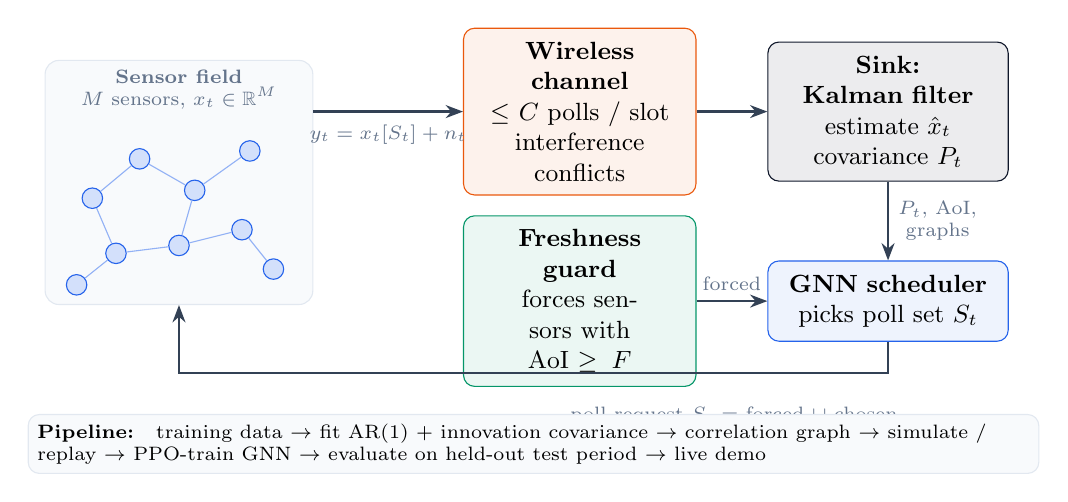
\begin{tikzpicture}[node distance=0.55cm and 0.75cm]
    % sensor field
    \node[draw=rule,fill=paper,rounded corners=5pt,minimum width=3.4cm,minimum height=3.1cm] (field) {};
    \node[lab,anchor=north] at (field.north) {\textbf{Sensor field}\\ $M$ sensors, $x_t\in\mathbb{R}^M$};
    \foreach \x/\y [count=\i] in {-1.1/-0.2,-0.5/0.3,0.2/-0.1,0.9/0.4,-0.8/-0.9,0.0/-0.8,0.8/-0.6,1.2/-1.1,-1.3/-1.3}
      \node[circle,draw=accent,fill=accent!20,minimum size=0.26cm,inner sep=0] (n\i) at ($(field.center)+(\x,\y)$) {};
    \draw[accent!50] (n1)--(n2)--(n3)--(n4) (n1)--(n5)--(n6)--(n3) (n6)--(n7)--(n8) (n5)--(n9);

    \node[box=orangeb,right=1.9cm of field,text width=2.6cm,yshift=0.9cm] (chan) {\textbf{Wireless channel}\\ $\le C$ polls / slot\\ interference conflicts};
    \node[box=ink,right=0.9cm of chan,text width=2.7cm] (sink) {\textbf{Sink: Kalman filter}\\ estimate $\hat x_t$\\ covariance $P_t$};
    \node[box=accent,below=1.0cm of sink,text width=2.7cm] (gnn) {\textbf{GNN scheduler}\\ picks poll set $S_t$};
    \node[box=good,left=0.9cm of gnn,text width=2.6cm] (guard) {\textbf{Freshness guard}\\ forces sensors with\\ AoI $\ge F$};

    \draw[arr] (field.east|-chan.west) -- node[lab,below,yshift=-1pt]{$y_t=x_t[S_t]+n_t$} (chan.west);
    \draw[arr] (chan) -- (sink);
    \draw[arr] (sink) -- node[lab,right]{$P_t$, AoI,\\ graphs} (gnn);
    \draw[arr] (guard) -- node[lab,above]{forced} (gnn);
    \draw[arr] (gnn.south) -- ++(0,-0.4) -| (field.south);
    \node[lab,anchor=north] at ($(gnn.south)!0.5!(guard.south)+(0,-0.42)$) {poll request $S_t$ = forced $\cup$ chosen};

    \node[draw=rule,fill=paper,rounded corners=4pt,anchor=north,text width=12.6cm,font=\scriptsize,align=left]
      at ($(field.south)!0.5!(gnn.south)+(0,-1.15)$)
      {\textbf{Pipeline:}\quad training data $\rightarrow$ fit AR(1) + innovation covariance $\rightarrow$ correlation graph
      $\rightarrow$ simulate / replay $\rightarrow$ PPO-train GNN $\rightarrow$ evaluate on held-out test period $\rightarrow$ live demo};
  \end{tikzpicture}
\end{frame}

% =================================================================== 9 MODEL
\begin{frame}{Methodology (2/5): Correlation Graph and Kalman Sink}
  \begin{columns}[T]
    \begin{column}{0.52\textwidth}
      \sect{Field model, fitted on the training period only}
      \vspace{-0.6em}
      \begin{align*}
        x_t &= \operatorname{diag}(\rho)\,x_{t-1} + w_t, & w_t &\sim \mathcal N(0,Q)\\
        y_t &= x_t[S_t] + n_t, & n_t &\sim \mathcal N(0,rI)
      \end{align*}
      \begin{itemize}\small
        \item $\rho_i$: least squares on one-step changes, per sensor
        \item $Q$: covariance of the residuals (innovations)
      \end{itemize}
      \sect{Correlation graph}
      \vspace{-0.4em}
      \[ (A_{\text{corr}})_{ij} = |\hat r_{ij}|\cdot\mathbf{1}\big[\,|\hat r_{ij}|\ge 0.3\,\big] \]
      {\small $\hat r$ = innovation correlation. Edges link sensors whose \emph{surprises} move together.}
    \end{column}
    \begin{column}{0.46\textwidth}
      \sect{Sink: Kalman filter}
      \vspace{-0.6em}
      \begin{align*}
        P^-_t &= D\,P_{t-1}\,D + Q,\qquad D=\operatorname{diag}(\rho)\\
        P_t &= P^-_t - P^-_{:,S}\big(P^-_{SS}+rI\big)^{-1}P^-_{S,:}
      \end{align*}
      \begin{block}{Why this matters}
        \small Polling sensor $j$ lowers $P_{ii}$ for every \emph{correlated} neighbour $i$.
        The variance removed by polling $i$ next is
        \[ g_i = \frac{\sum_k P_{ki}^2}{P_{ii}+r}, \]
        which drives both the Kalman-greedy baseline \cite{19} and our decoder.
      \end{block}
    \end{column}
  \end{columns}
\end{frame}

% =================================================================== 10 FORMULATION
\begin{frame}{Methodology (3/5): Formulation and Freshness Guarantee}
  \begin{columns}[T]
    \begin{column}{0.55\textwidth}
      \sect{Objective}
      \vspace{-0.4em}
      \[
        \min_{\pi}\; \mathbb E\Big[\tfrac{1}{TM}\textstyle\sum_{t=1}^{T}\lVert x_t-\hat x_t\rVert^2\Big]
      \]
      \vspace{-0.6em}
      \sect{subject to, in every slot $t$}
      \begin{itemize}\small
        \item capacity: $|S_t|\le C$
        \item interference: no two conflicting sensors in $S_t$
        \item \textbf{freshness}: $a_i(t)\le F$ for every sensor $i$
      \end{itemize}
      \sect{Age of Information}
      \vspace{-0.5em}
      \[
        a_i(t+1)=\begin{cases}1 & i\in S_t\\ a_i(t)+1 & \text{otherwise}\end{cases}
      \]
    \end{column}
    \begin{column}{0.43\textwidth}
      \sect{Freshness guard (hard, every policy)}
      \begin{enumerate}\small\setlength\itemsep{0.3em}
        \item Forced set $\mathcal F_t=\{i: a_i(t)\ge F\}$, oldest first, conflict-feasible.
        \item Forced sensors are committed \emph{before} the policy acts.
        \item The policy fills the remaining $C-|\mathcal F_t|$ slots.
        \item The environment asserts capacity, conflicts and freshness each step.
      \end{enumerate}
      \vspace{0.3em}
      \begin{block}{Setting}
        \small $F=\lfloor 3M/C\rfloor$ \; (Intel: 22 slots = 1.8\,h; PEMS-BAY: 24 slots = 2\,h).
        The policy is a Markov decision process over the sink's state, solved with PPO.
      \end{block}
    \end{column}
  \end{columns}
\end{frame}

% =================================================================== 11 ARCHITECTURE
\begin{frame}{Methodology (4/5): GNN Scheduler Architecture}
  \centering
  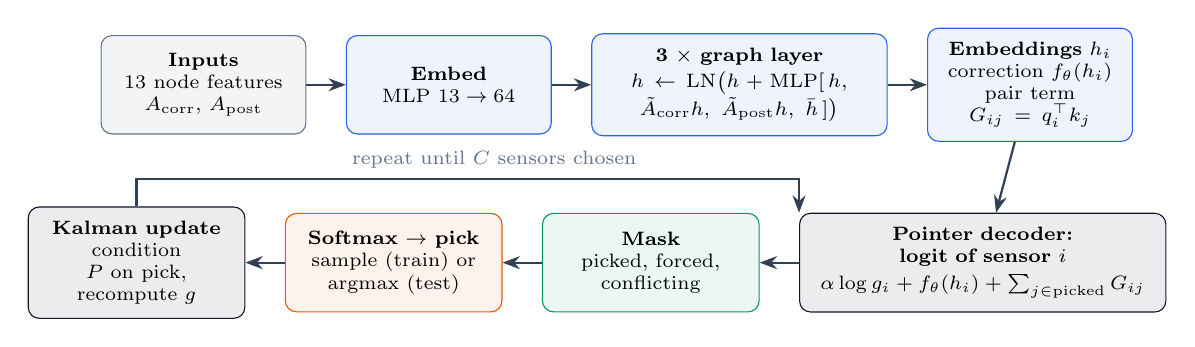
\begin{tikzpicture}[node distance=0.45cm and 0.5cm]
    \node[st=muted] (in) {\textbf{Inputs}\\ 13 node features\\ $A_{\text{corr}}$, $A_{\text{post}}$};
    \node[st=accent,right=of in] (emb) {\textbf{Embed}\\ MLP $13\!\to\!64$};
    \node[st=accent,right=of emb,text width=3.4cm] (mp) {\textbf{3 $\times$ graph layer}\\[0.2em] $h\leftarrow\mathrm{LN}\big(h+\mathrm{MLP}[\,h,$\\ $\tilde A_{\text{corr}}h,\ \tilde A_{\text{post}}h,\ \bar h\,]\big)$};
    \node[st=accent,right=of mp] (h) {\textbf{Embeddings} $h_i$\\ correction $f_\theta(h_i)$\\ pair term $G_{ij}=q_i^{\top}k_j$};
    \node[st=ink,below=0.9cm of h,text width=4.3cm,xshift=-0.6cm] (logit) {\textbf{Pointer decoder: logit of sensor $i$}\\[0.2em]
       $\alpha\log g_i + f_\theta(h_i) + \textstyle\sum_{j\in\text{picked}} G_{ij}$};
    \node[st=good,left=of logit,text width=2.4cm] (mask) {\textbf{Mask}\\ picked, forced,\\ conflicting};
    \node[st=orangeb,left=of mask,text width=2.4cm] (pick) {\textbf{Softmax $\rightarrow$ pick}\\ sample (train) or\\ argmax (test)};
    \node[st=ink,left=of pick,text width=2.4cm] (kal) {\textbf{Kalman update}\\ condition $P$ on pick,\\ recompute $g$};

    \draw[arr] (in)--(emb); \draw[arr] (emb)--(mp); \draw[arr] (mp)--(h); \draw[arr] (h)--(logit);
    \draw[arr] (logit)--(mask); \draw[arr] (mask)--(pick); \draw[arr] (pick)--(kal);
    \draw[arr] (kal.north) -- ++(0,0.35) -| node[lab,pos=0.27,above]{repeat until $C$ sensors chosen} (logit.north west);
  \end{tikzpicture}
  \vspace{0.4em}
  \begin{columns}[T]
    \begin{column}{0.5\textwidth}
      \begin{itemize}\scriptsize
        \item Features: AoI, last polled, posterior variance (and log), gain $g_i$ (and log),
              forced flag, freshness slack, $C/M$, $\hat\rho_i$, drift rate, graph degree, guard on/off.
        \item $A_{\text{post}}=|P_{ij}|/\sqrt{P_{ii}P_{jj}}$: who is redundant \emph{right now}.
      \end{itemize}
    \end{column}
    \begin{column}{0.48\textwidth}
      \begin{itemize}\scriptsize
        \item \textbf{Residual design}: $f_\theta$ and $G$ start at zero, so the untrained actor
              \emph{is} Kalman-greedy (unit-tested).
        \item Plackett--Luce product of softmaxes gives exact log-probabilities for PPO.
        \item 137k parameters; works for any $M$ (shared weights).
      \end{itemize}
    \end{column}
  \end{columns}
\end{frame}

% =================================================================== 12 PPO
\begin{frame}[fragile]{Methodology (5/5): Training with PPO}
  \begin{columns}[T]
    \begin{column}{0.58\textwidth}
      \begin{algorithm}[H]
        \scriptsize
        \caption{\small PPO training of the GNN scheduler}
        \begin{algorithmic}[1]
          \State Initialise actor $\pi_\theta$ = Kalman-greedy ($f_\theta{=}G{=}0$), critic $V_\phi$
          \For{iteration $=1,\dots,N$}
            \State Sample batch of envs: synthetic ($M\!\in\![10,100]$, random $C$, layout, $\rho$, $F$)
            \Statex \hspace{1.2em} or, with prob.\ 0.35, real training-period replays
            \For{$t=1,\dots,96$}
              \State $\mathcal F_t\gets$ freshness guard; $S_t\gets\mathcal F_t\cup\pi_\theta(\text{features},A_{\text{corr}},A_{\text{post}})$
              \State Step env; reward $r_t=-(1-\gamma)\log(\text{error}_t+0.005)$
            \EndFor
            \State Advantages $\hat A_t$ with GAE ($\gamma=0.95,\lambda=0.9$)
            \For{4 epochs, minibatches of 512}
              \State $\eta_t=\pi_\theta(S_t)/\pi_{\theta_{\text{old}}}(S_t)$ \Comment{Plackett--Luce}
              \State $L=-\min(\eta_t\hat A_t,\operatorname{clip}(\eta_t,0.85,1.15)\hat A_t)-0.002\,\mathcal H$
              \State Adam step on $\theta$; regress $V_\phi$ to returns
            \EndFor
            \State Every 10 iters: validate; keep best checkpoint
          \EndFor
        \end{algorithmic}
      \end{algorithm}
    \end{column}
    \begin{column}{0.4\textwidth}
      \sect{Why these choices}
      \begin{itemize}\small\setlength\itemsep{0.4em}
        \item \textbf{Greedy start}: PPO begins from the strongest model-based scheduler instead of random.
        \item \textbf{Log reward} balances small and large networks in one batch.
        \item \textbf{Real replays}: the sink is fitted on the first 70\% of the training period and
              episodes run on the next 20\%, so the policy learns to cope with model mismatch.
        \item Last 10\% of training data + seeds $\ge 9000$ for validation; test periods and
              layouts ($\ge 10000$) are never seen.
      \end{itemize}
    \end{column}
  \end{columns}
\end{frame}

\section{Implementation}

% =================================================================== 13 IMPLEMENTATION: STACK
\begin{frame}[fragile]{Implementation (1/5): Tech Stack and Code Structure}
  \begin{columns}[T]
    \begin{column}{0.44\textwidth}
      \sect{Stack}
      \begin{itemize}\small\setlength\itemsep{0.35em}
        \item \textbf{Python 3.13}, NumPy, PyTorch (CPU)
        \item Dense batched message passing (no graph library needed at $M\le 325$)
        \item Matplotlib for figures and the animated GIF
        \item Standard-library HTTP server + vanilla JavaScript/Canvas front end
        \item pytest (21 tests) on GitHub Actions CI
        \item Open source on GitHub:\\ {\scriptsize\texttt{BhanuPrasadPalella-01/gnn-aoi-scheduler}}
      \end{itemize}
    \end{column}
    \begin{column}{0.54\textwidth}
      \sect{Repository layout}
      \scriptsize
\begin{verbatim}
gnn_aoi/
  simulator.py   correlated field, fit_model
  datasets.py    Intel Lab, PEMS-BAY loaders
  graphs.py      correlation & interference
  estimator.py   Kalman sink
  env.py         slots, AoI, freshness guard
  policies/      5 baselines + GNN policy
  gnn/           features, model, PPO train
  experiments.py benchmarks, sweeps, stats
  live.py        step-by-step live session
  server.py      HTTP API for the demo
frontend/        live dashboard (JS/Canvas)
tests/           21 unit/regression tests
\end{verbatim}
    \end{column}
  \end{columns}
\end{frame}

% =================================================================== 14 DATASETS
\begin{frame}{Implementation (2/5): Real Datasets and Preprocessing}
  \small
  \begin{tabularx}{\textwidth}{@{}l>{\raggedright\arraybackslash}X>{\raggedright\arraybackslash}X@{}}
    \toprule
     & \textbf{Intel Berkeley Research Lab} \cite{25} & \textbf{PEMS-BAY} \cite{24} \\
    \midrule
    Quantity & Indoor temperature ($^\circ$C) & Freeway traffic speed (mph) \\
    Sensors $M$ & 45 (after quality filtering) & 325 loop detectors \\
    Slot & 5 min & 5 min \\
    Capacity $C$ / bound $F$ & 6 polls / 22 slots & 40 polls / 24 slots \\
    Train period & 28 Feb -- 8 Mar 2004 & Jan -- Apr 2017 \\
    Test period & 9 -- 18 Mar 2004 (10 windows $\times$ 200 slots) & May -- Jun 2017 (15 windows $\times$ 288 slots) \\
    Daily profile removed & time of day & time of day, weekday / weekend \\
    \bottomrule
  \end{tabularx}
  \vspace{0.6em}
  \begin{itemize}\small\setlength\itemsep{0.2em}
    \item Standardised with training-period statistics only; no test data leaks into the model (unit-tested).
    \item Intel data has \textbf{recording outages} (10--11 and 15--16 Mar): episodes never cross a gap.
    \item float32 storage and pre-fitted models cut memory from $\approx$1.75\,GB to $\approx$200--400\,MB.
  \end{itemize}
\end{frame}

% =================================================================== 15 TRAINING SETUP
\begin{frame}{Implementation (3/5): Training Setup}
  \begin{columns}[T]
    \begin{column}{0.36\textwidth}
      \scriptsize
      \begin{tabular}{@{}ll@{}}
        \toprule
        \textbf{Hyper-parameter} & \textbf{Value} \\
        \midrule
        Embedding size / layers & 64 / 3 \\
        Envs per batch & 32 (at $M{=}40$) \\
        Rollout length & 96 slots \\
        PPO iterations & 400 \\
        $\gamma$ / GAE $\lambda$ & 0.95 / 0.9 \\
        Clip $\epsilon$ & 0.15 \\
        Epochs / minibatch & 4 / 512 \\
        LR actor / critic & $10^{-4}$ / $5\!\times\!10^{-4}$ \\
        Entropy coef. & 0.002 \\
        Real-data share & 35\% \\
        Hardware & laptop CPU \\
        Training time & $\approx$35 min \\
        \bottomrule
      \end{tabular}
    \end{column}
    \begin{column}{0.62\textwidth}
      \centering
      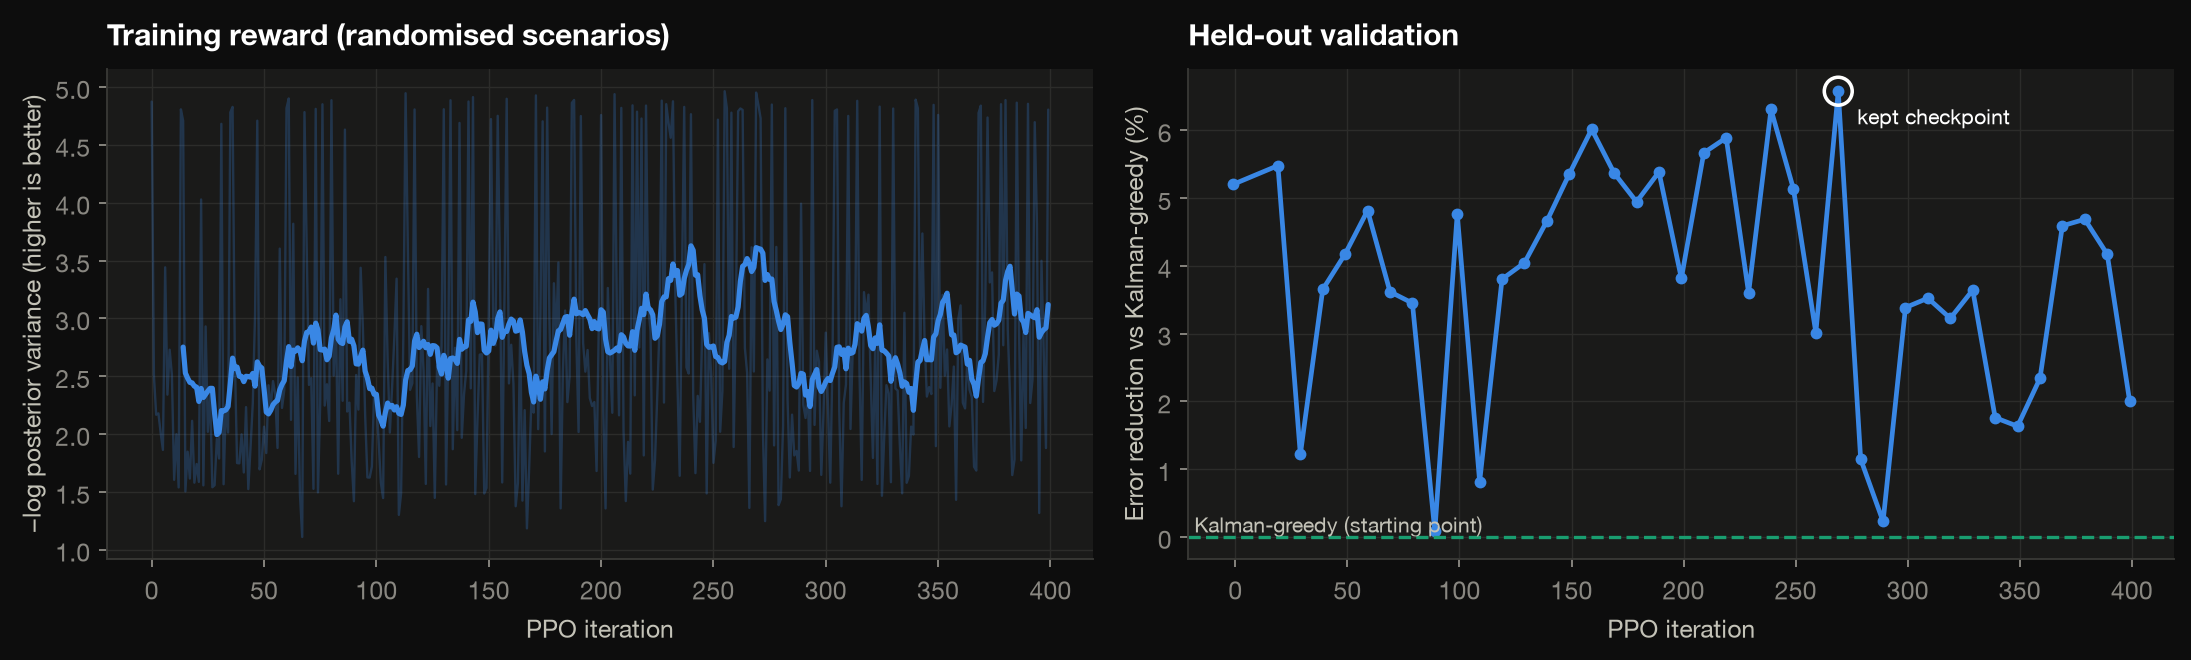
\includegraphics[width=\textwidth]{figures/training.png}\\[0.4em]
      \begin{itemize}\scriptsize
        \item Left: training reward over randomised scenarios (noisy by design: every batch is a different network).
        \item Right: held-out validation error vs.\ Kalman-greedy, which is exactly where training starts (0\%).
              The best checkpoint is kept (\good{+6.6\%} better than Kalman-greedy).
        \item Training is resumable and was warm-started from an earlier run.
      \end{itemize}
    \end{column}
  \end{columns}
\end{frame}

% =================================================================== 16 BASELINES
\begin{frame}{Implementation (4/5): Baselines and Evaluation Protocol}
  \begin{columns}[T]
    \begin{column}{0.52\textwidth}
      \sect{Schedulers (same freshness guard for all)}
      \footnotesize
      \begin{tabularx}{\textwidth}{@{}l>{\raggedright\arraybackslash}X@{}}
        \toprule
        \textbf{Max-AoI (B1)} & poll the stalest sensors: AoI-based scheduling \cite{2,16} \\
        \textbf{Random} & uniform choice \\
        \textbf{Corr-diverse (v4)} & stalest first, discount neighbours by $|$correlation$|$ \\
        \textbf{Max-uncertainty} & largest posterior variance $P_{ii}$ \\
        \textbf{Kalman-greedy} & greedy variance reduction on the sink's covariance \cite{19} \\
        \textbf{Oracle-greedy} & Kalman-greedy with the \emph{true} covariance (synthetic only) \\
        \textbf{Ablation} & GNN with message passing removed \\
        \bottomrule
      \end{tabularx}
    \end{column}
    \begin{column}{0.45\textwidth}
      \sect{Protocol}
      \begin{itemize}\small\setlength\itemsep{0.35em}
        \item \textbf{Metric}: sink estimation error (RMSE in $^\circ$C / mph; MSE in standardised units).
        \item \textbf{Real data}: held-out test windows only.
        \item \textbf{Synthetic}: 30 unseen layouts $\times$ 350 slots, uniform and clustered.
        \item \textbf{Statistics}: mean $\pm$ 95\% CI, per-window win rate, Wilcoxon signed-rank test.
        \item Sweeps over capacity $C$, network size $M$, interference, freshness on/off.
        \item Decision time per slot measured on CPU.
      \end{itemize}
    \end{column}
  \end{columns}
\end{frame}

% =================================================================== 17 DEMO
\begin{frame}{Implementation (5/5): Live Transmission Demo}
  \begin{columns}[c]
    \begin{column}{0.68\textwidth}
      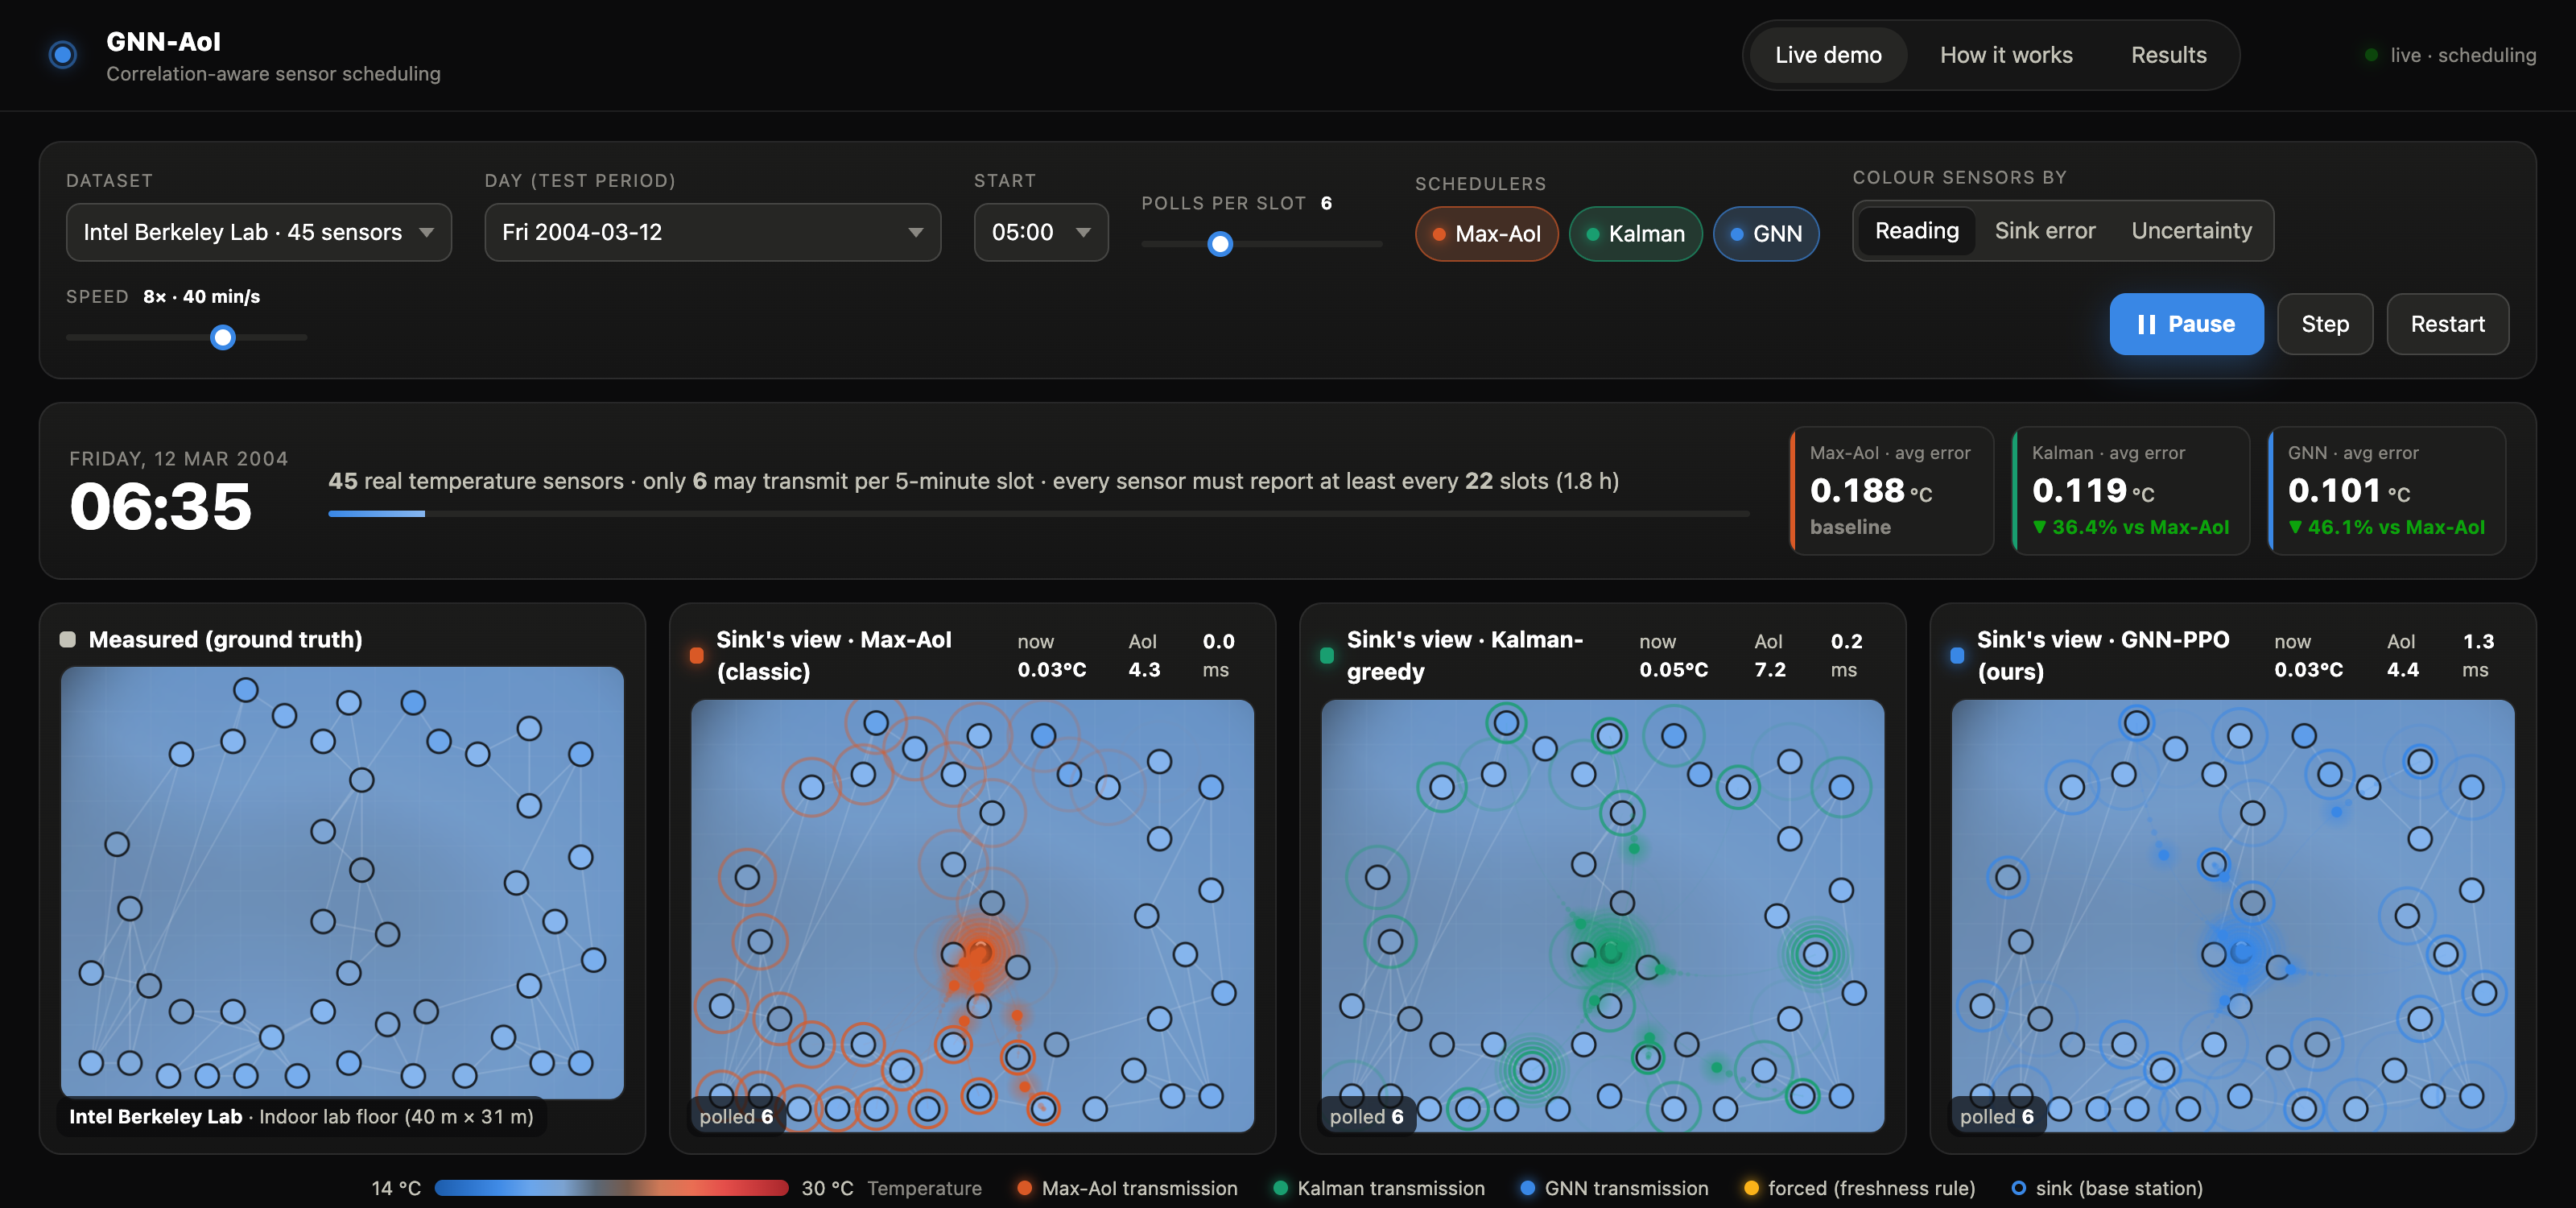
\includegraphics[width=\textwidth]{figures/live_demo.png}
    \end{column}
    \begin{column}{0.3\textwidth}
      \begin{itemize}\scriptsize\setlength\itemsep{0.4em}
        \item Replays a \textbf{real test day} slot by slot (here Intel Lab, 12 Mar 2004).
        \item Three schedulers run side by side on the same readings; rings = sensors polled this slot.
        \item Each map shows the \textbf{sink's view}: what it believes the field looks like.
        \item ``Why these sensors?'' shows the GNN's pick probabilities; the log lists every transmission.
        \item Runs locally: \texttt{python -m gnn\_aoi serve}, then open \texttt{localhost:8000}.
      \end{itemize}
    \end{column}
  \end{columns}
\end{frame}

\section{Results and Discussion}

% =================================================================== 18 RESULTS REAL
\begin{frame}{Results (1/5): Real Sensor Data, Held-out Test Periods}
  \centering
  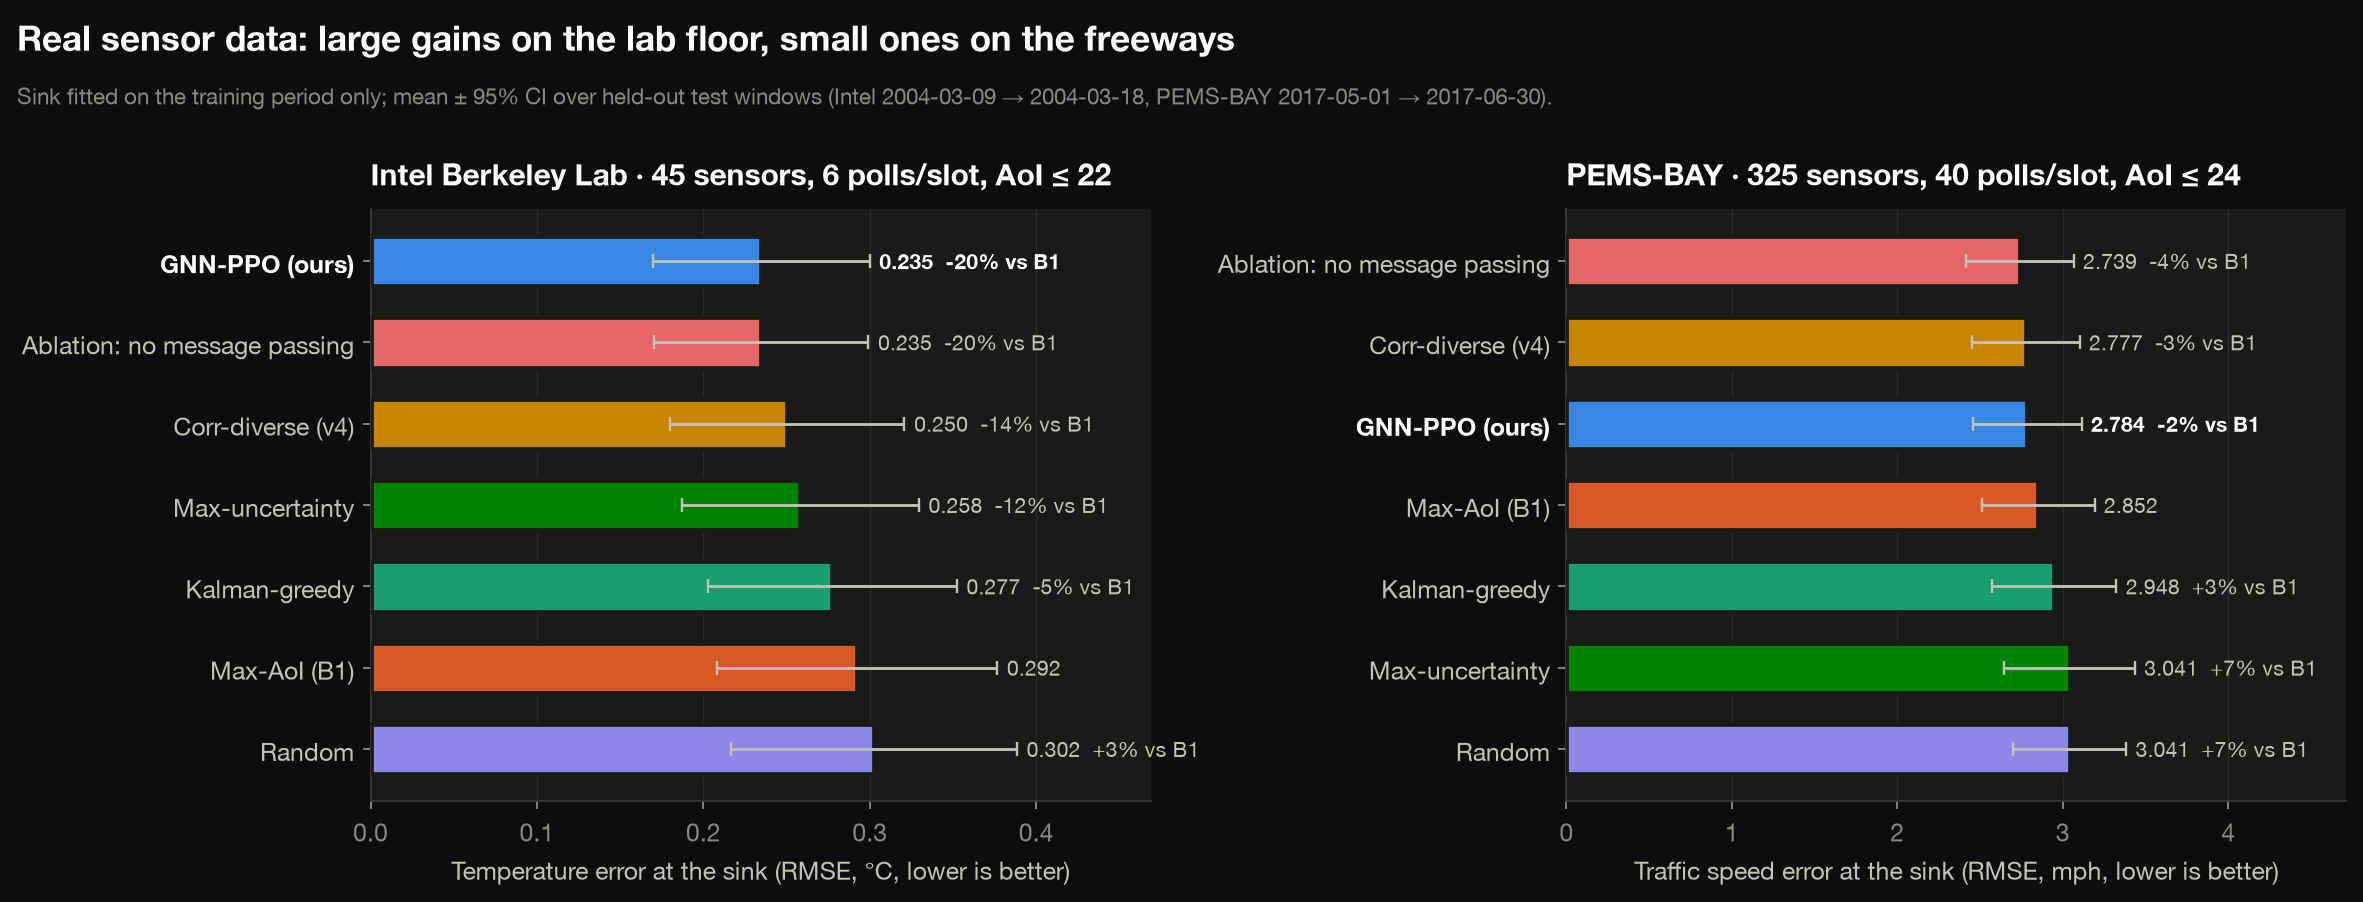
\includegraphics[width=0.93\textwidth]{figures/real_benchmark.png}\\[0.2em]
  \begin{columns}[T]
    \begin{column}{0.49\textwidth}
      \begin{itemize}\scriptsize
        \item \textbf{Intel Lab}: GNN \good{0.235\,$^\circ$C} vs.\ Max-AoI 0.292 (\good{$-20\%$}) and Kalman-greedy 0.277.
              GNN beats Kalman-greedy in \textbf{10/10} test windows ($p=0.002$).
      \end{itemize}
    \end{column}
    \begin{column}{0.49\textwidth}
      \begin{itemize}\scriptsize
        \item \textbf{PEMS-BAY}: GNN 2.78\,mph vs.\ Max-AoI 2.85 (\good{$-2.4\%$}); Kalman-greedy is \bad{worse} than
              Max-AoI here (2.95). GNN beats Kalman-greedy in \textbf{15/15} windows ($p=6\times10^{-5}$).
      \end{itemize}
    \end{column}
  \end{columns}
\end{frame}

% =================================================================== 19 SWEEPS
\begin{frame}{Results (2/5): Capacity and Size Sweeps, Real Data}
  \centering
  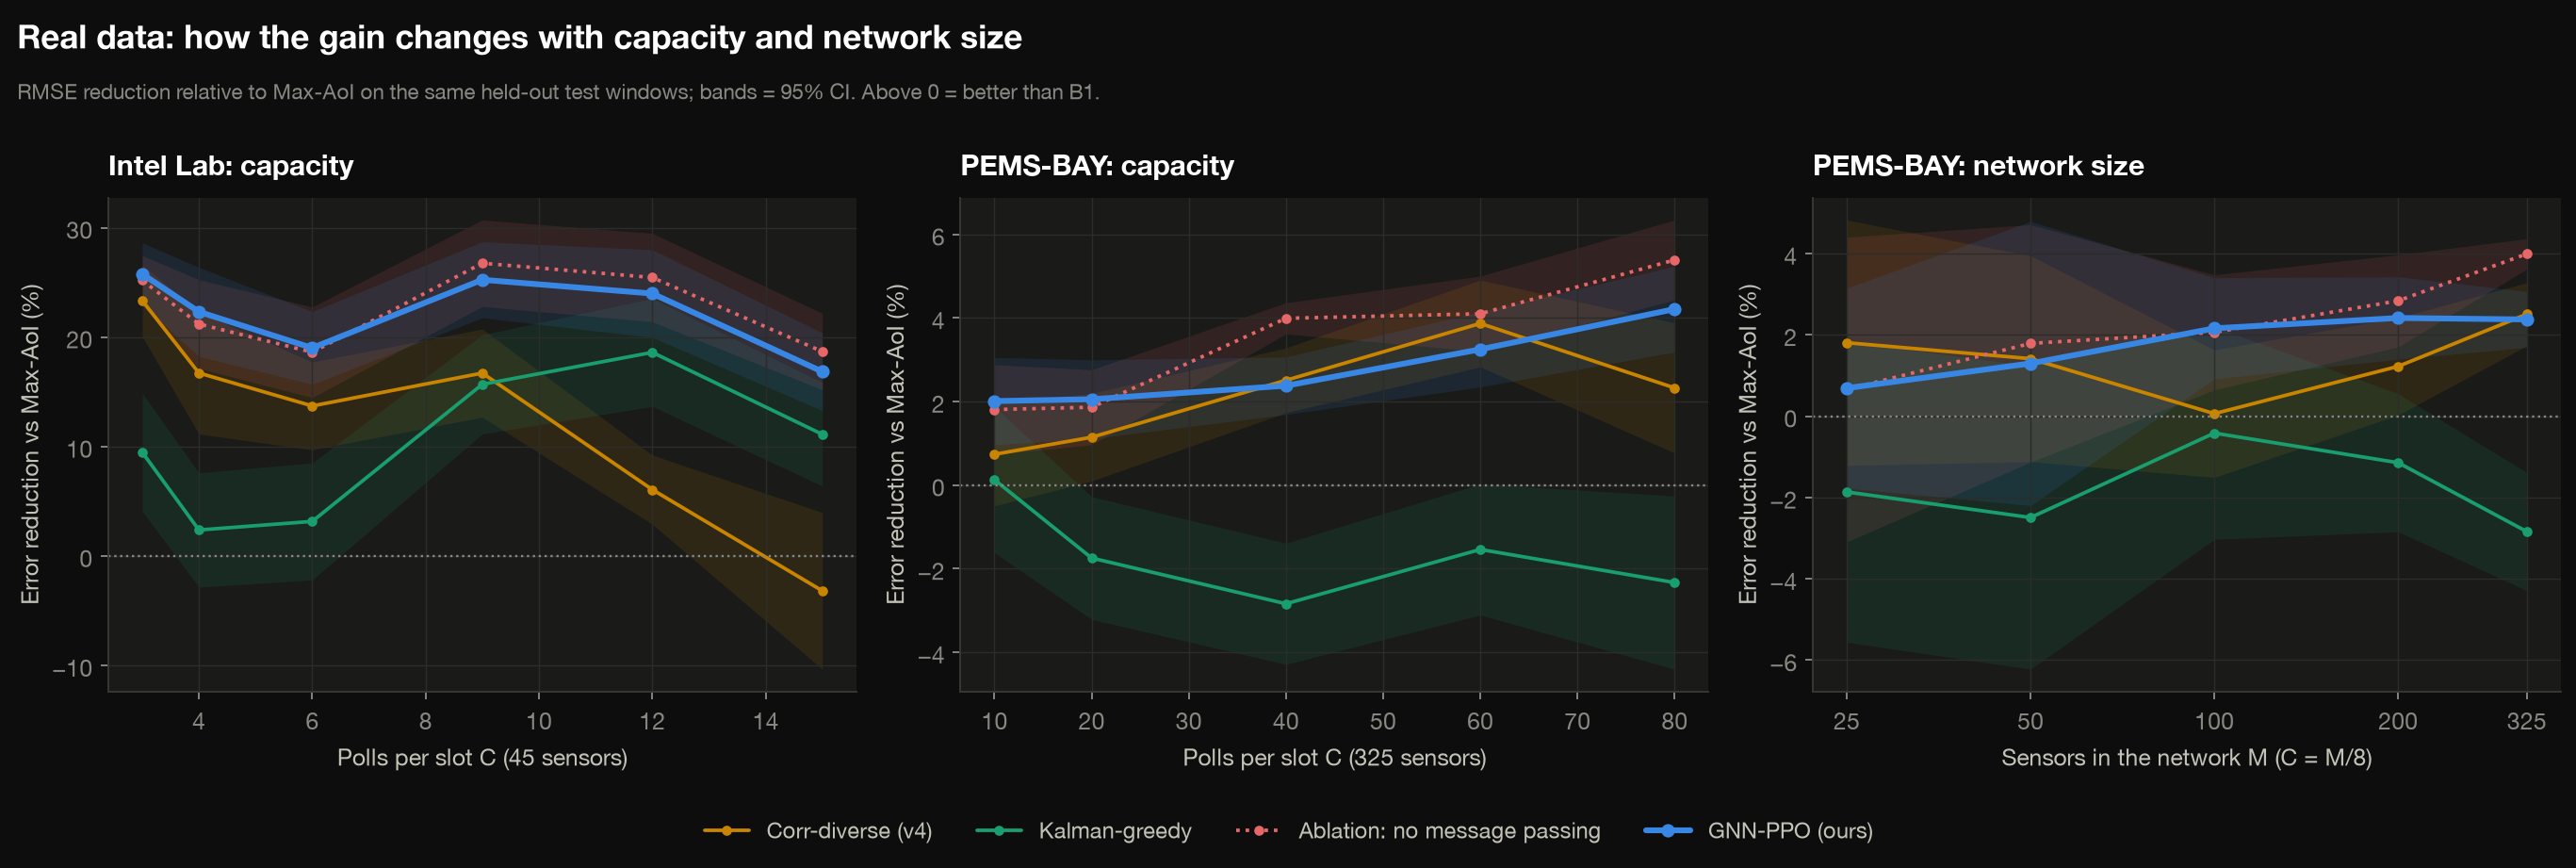
\includegraphics[width=0.95\textwidth]{figures/real_sweeps.png}\\[0.3em]
  \begin{itemize}\small\setlength\itemsep{0.3em}
    \item Intel Lab: GNN stays \good{17--26\%} below Max-AoI for every capacity $C=3\dots15$; Kalman-greedy and the
          correlation heuristic are inconsistent (the heuristic even loses at $C=15$).
    \item PEMS-BAY: the gain grows with capacity (2\% $\rightarrow$ 4\%) and network size; Kalman-greedy is
          \bad{below} Max-AoI for most settings because its fitted model is over-confident on freeway data.
  \end{itemize}
\end{frame}

% =================================================================== 20 SYNTHETIC
\begin{frame}{Results (3/5): Synthetic Data, Ablation, Freshness}
  \begin{columns}[T]
    \begin{column}{0.62\textwidth}
      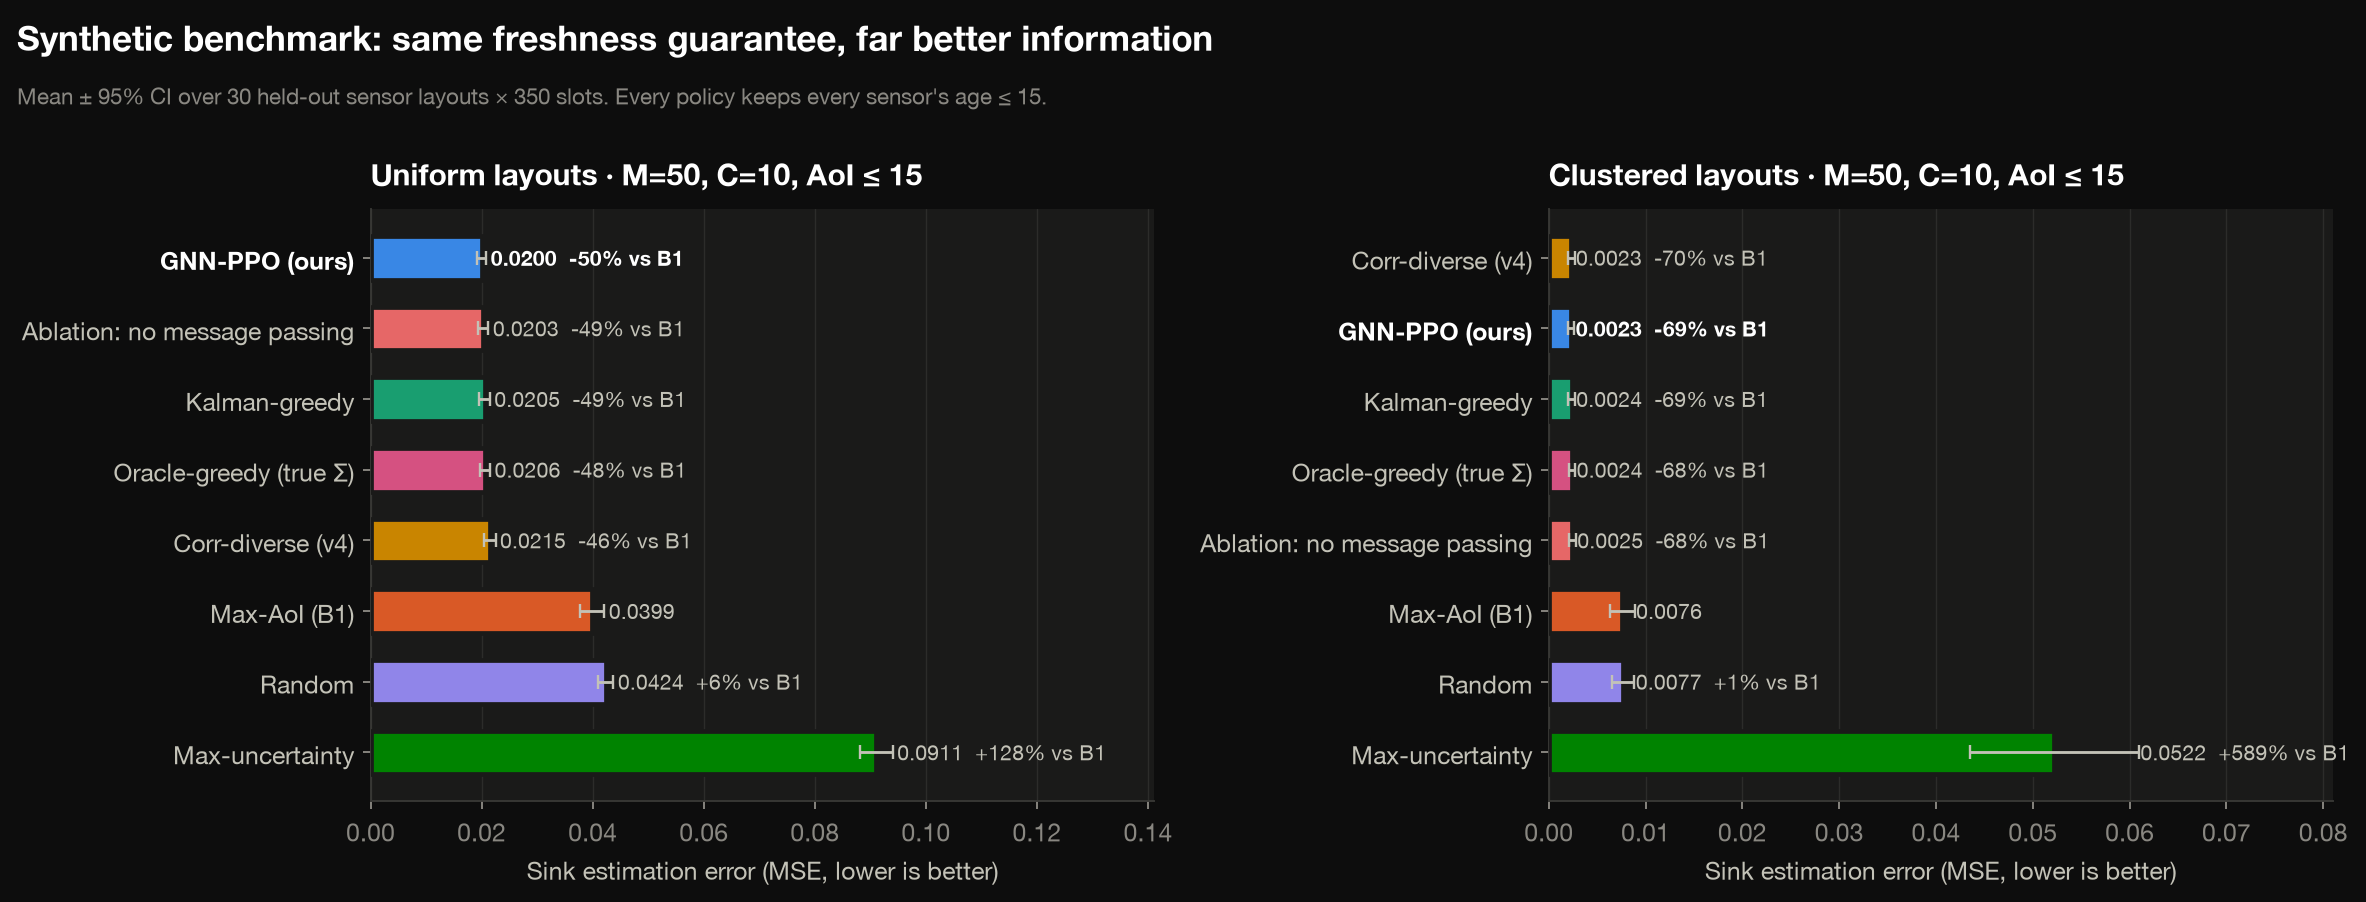
\includegraphics[width=\textwidth]{figures/main_benchmark.png}
      \begin{itemize}\scriptsize
        \item Uniform: GNN \good{$-50\%$} MSE vs.\ Max-AoI; beats Kalman-greedy on 73\% of layouts ($p=0.008$) and
              \textbf{oracle-greedy with the true covariance} on 70\% ($p=0.003$).
        \item Clustered: all correlation-aware policies tie ($\approx-69\%$ vs.\ Max-AoI).
        \item Ablation: message passing helps on synthetic layouts (wins 67\% uniform, 87\% clustered).
      \end{itemize}
    \end{column}
    \begin{column}{0.36\textwidth}
      \sect{Freshness guard switched off ($M{=}50$, $C{=}10$)}
      \scriptsize
      \begin{tabular}{@{}lccc@{}}
        \toprule
        Policy & MSE & Starved & Max AoI \\
        \midrule
        Max-AoI & 0.0399 & 0 & 5 \\
        Kalman-greedy & 0.0229 & \bad{18} & \bad{401} \\
        Oracle-greedy & 0.0226 & \bad{19.6} & \bad{401} \\
        \textbf{GNN (ours)} & \good{0.0200} & \good{0} & 10.3 \\
        \bottomrule
      \end{tabular}\\[0.5em]
      {\scriptsize Greedy variance reduction \textbf{abandons} sensors it can infer from neighbours (never polled
      in 400 slots). The GNN gets lower error \emph{and} polls everyone, even without the guard.}
    \end{column}
  \end{columns}
\end{frame}

% =================================================================== 21 COMPARISON WITH LITERATURE
\begin{frame}{Results (4/5): Comparison with Recent Literature}
  \scriptsize
  \begin{tabularx}{\textwidth}{@{}>{\raggedright\arraybackslash}p{2.6cm}>{\raggedright\arraybackslash}p{3.0cm}YY@{}}
    \toprule
    \textbf{Work} & \textbf{Approach} & \textbf{Reported in their own setting} & \textbf{Same approach, measured on our real data} \\
    \midrule
    Ramakanth \emph{et al.}\ \cite{2}, INFOCOM 2024; Kadota \emph{et al.}\ \cite{16}
      & AoI-based (max-age) scheduling, correlation ignored
      & Provably within a constant factor of optimal (Wiener model, 1 source / slot)
      & Our Max-AoI (B1): GNN lowers RMSE \good{20\%} (Intel) and \good{2.4\%} (PEMS-BAY); wins 10/10 and 15/15 windows \\
    \addlinespace
    Chen \emph{et al.}\ \cite{8}, ICC 2023
      & Structure-enhanced DRL for remote-estimation MSE
      & 10--25\% lower MSE than benchmark DRL; 50\% less training time
      & GNN: \good{25.8\%} lower MSE than Kalman-greedy (Intel), \good{13.4\%} (PEMS-BAY); trains in $\approx$35\,min on a CPU \\
    \addlinespace
    Krause \emph{et al.}\ \cite{19} (greedy variance reduction)
      & Submodular greedy sensor selection
      & Near-optimal one-step selection
      & GNN beats it in 73\% of synthetic layouts and beats it \emph{with the true covariance} in 70\% \\
    \addlinespace
    Reyhan \& Coleri \cite{9}, TCOM 2025; Farag \emph{et al.}\ \cite{7}
      & DRL with AoI-violation \emph{probability} constraints
      & Constraints satisfied in probability
      & \textbf{Hard} bound: zero violations by construction; unconstrained greedy starves 18/50 sensors \\
    \bottomrule
  \end{tabularx}
  \vspace{0.5em}

  {\scriptsize\color{muted} Numbers in the third column come from the cited papers' own setups and are not
  directly comparable; the fourth column re-runs that \emph{class} of method on our held-out data under identical conditions.}
\end{frame}

% =================================================================== 22 DISCUSSION
\begin{frame}{Results (5/5): Discussion and Limitations}
  \begin{columns}[T]
    \begin{column}{0.56\textwidth}
      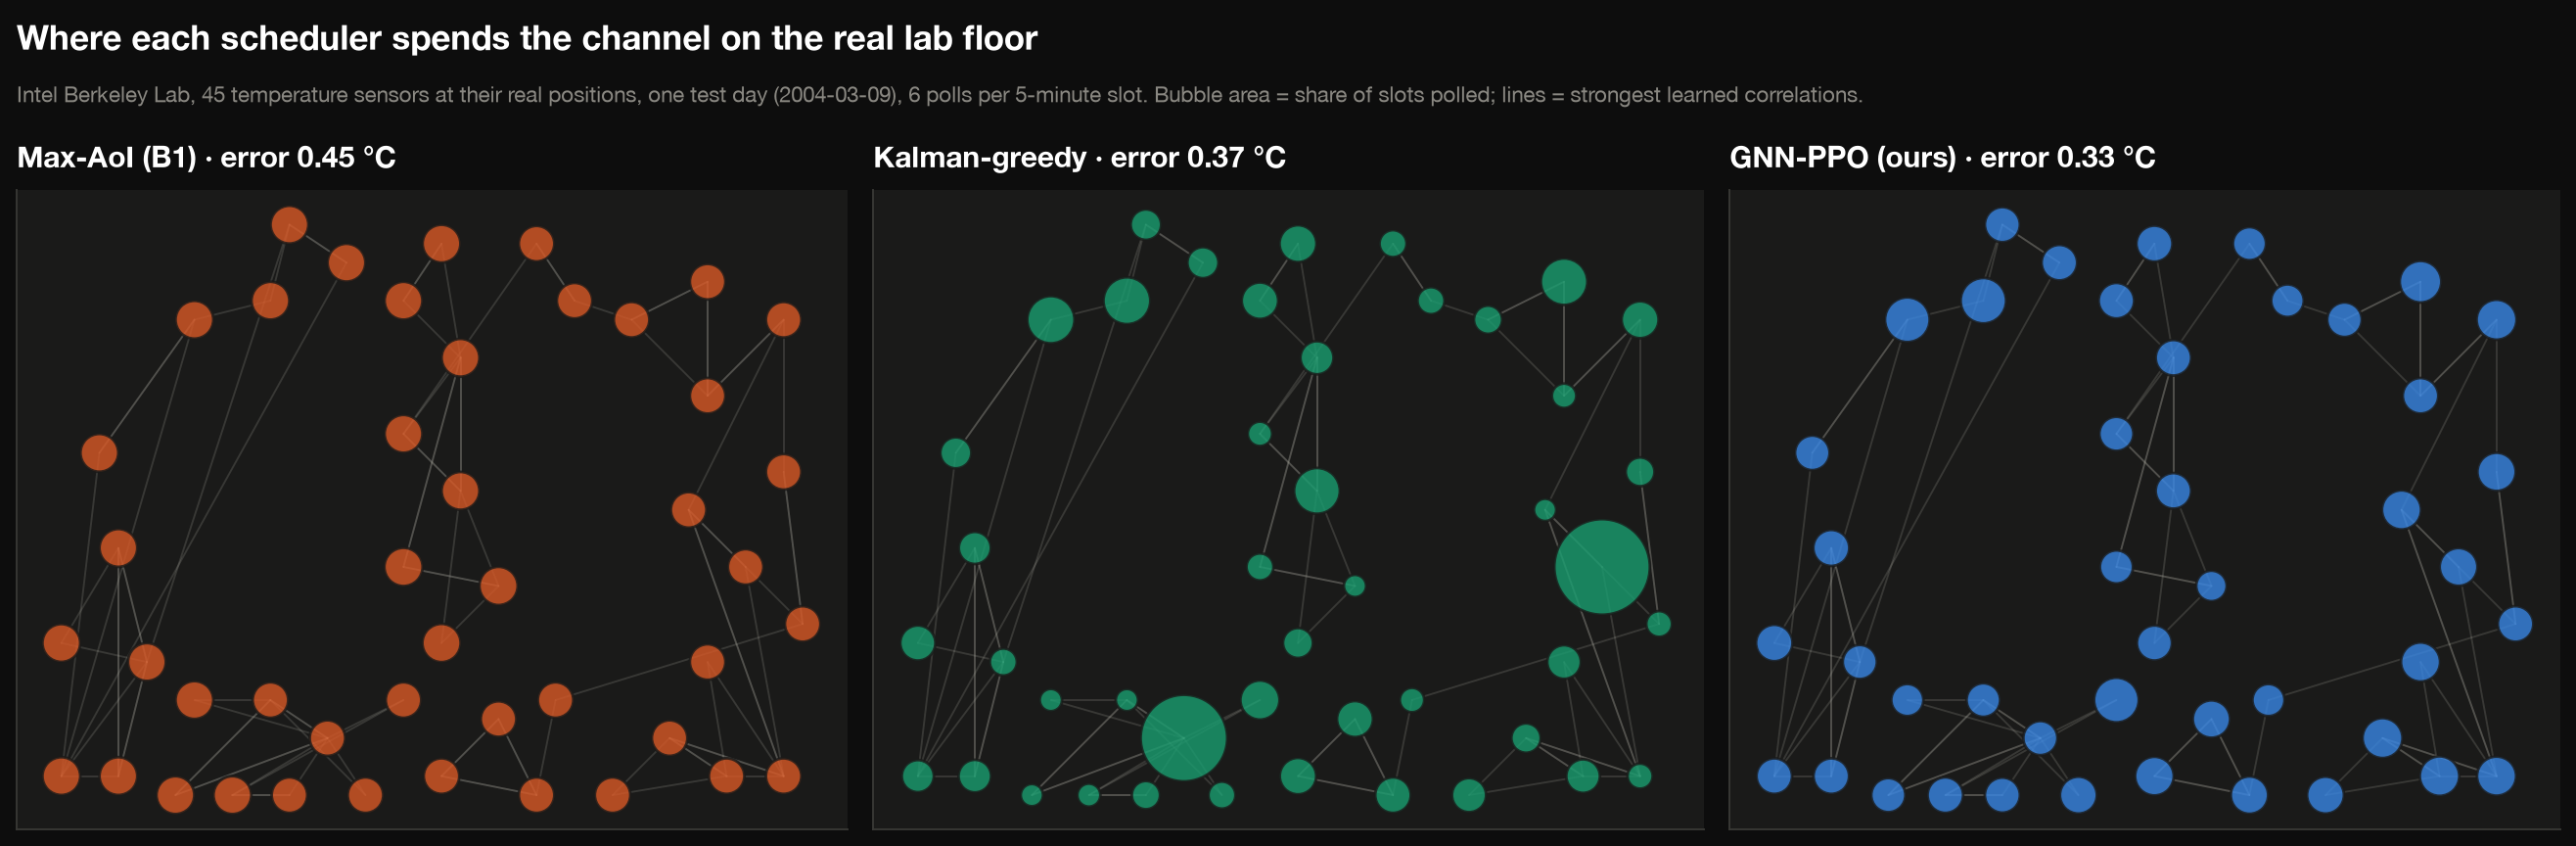
\includegraphics[width=\textwidth]{figures/poll_map.png}\\[-0.2em]
      {\scriptsize\color{muted} Bubble area = share of slots each sensor was polled (Intel Lab, one test day).
      Max-AoI is uniform; Kalman-greedy concentrates on a few ``hub'' sensors; the GNN spreads polls
      by redundancy.}
    \end{column}
    \begin{column}{0.42\textwidth}
      \sect{What the results say}
      \begin{itemize}\scriptsize\setlength\itemsep{0.25em}
        \item Correlation awareness pays most where sensors are \textbf{strongly redundant} (lab floor), less on freeways.
        \item The learned policy is \textbf{robust to model mismatch}: Kalman-greedy trusts a wrong model; PPO on real replays corrects for it.
        \item Fast: 4.6\,ms (Intel) and 37\,ms (PEMS-BAY) per decision vs.\ a 5-minute slot.
      \end{itemize}
      \sect{Limitations (honest)}
      \begin{itemize}\scriptsize\setlength\itemsep{0.25em}
        \item On real data the \textbf{no-message-passing ablation ties} the full GNN: the gain comes mostly from the
              learned residual decoder.
        \item Synthetic $M\ge100$: Kalman-greedy is 8--12\% better (training covered $M\le100$).
        \item Linear-Gaussian sink; ideal channel apart from capacity and conflicts.
      \end{itemize}
    \end{column}
  \end{columns}
\end{frame}

\section{Conclusion and Future Work}

% =================================================================== 23 CONCLUSION
\begin{frame}{Conclusion}
  \begin{itemize}\setlength\itemsep{0.7em}
    \item Built \textbf{GNN-AoI}: a scheduler that learns the sensors' correlation graph from data, tracks the field with a
          Kalman sink, and picks transmissions with a GNN pointer decoder trained by PPO.
    \item Every sensor stays fresh by construction (hard AoI bound), unlike probabilistic or penalty-based methods.
    \item On \textbf{real held-out data} it lowers the sink's error by \good{20\%} on 45 Intel Lab sensors and
          \good{2.4\%} on 325 PEMS-BAY sensors versus AoI-based scheduling, and beats Kalman-greedy in
          \textbf{every} test window on both datasets.
    \item On synthetic fields it halves the error of max-age scheduling and even beats greedy selection that
          knows the true covariance.
    \item Delivered as an open-source, tested package with reproducible experiments and a live browser demo of
          the transmissions.
  \end{itemize}
\end{frame}

% =================================================================== 24 FUTURE WORK
\begin{frame}{Future Work}
  \begin{columns}[T]
    \begin{column}{0.49\textwidth}
      \begin{itemize}\setlength\itemsep{0.6em}
        \item \textbf{Lossy channels}: packet errors and retransmissions (HARQ, as in \cite{6}).
        \item \textbf{Online adaptation}: re-fit the correlation graph as the field drifts (seasons, new sensors).
        \item \textbf{Bigger networks}: train on $M>100$ and use sparse message passing for thousands of sensors.
      \end{itemize}
    \end{column}
    \begin{column}{0.49\textwidth}
      \begin{itemize}\setlength\itemsep{0.6em}
        \item \textbf{Non-linear sinks}: replace the Kalman filter with a learned spatio-temporal predictor
              (e.g.\ graph-recurrent models \cite{24}).
        \item \textbf{Distributed scheduling}: each gateway decides locally with the same shared GNN.
        \item \textbf{Hardware pilot}: run the scheduler on a real LoRa / Zigbee testbed.
      \end{itemize}
    \end{column}
  \end{columns}
\end{frame}

\section{References}

% =================================================================== 25-26 REFERENCES
\begin{frame}{References (1/3)}
  \scriptsize
  \begin{enumerate}\setlength\itemsep{0.25em}
    \item[{[1]}] V.~Tripathi and E.~Modiano, ``Optimizing age of information with correlated sources,'' in \emph{Proc.\ ACM MobiHoc}, 2022, pp.~41--50; extended in \emph{IEEE/ACM Trans.\ Netw.}, vol.~32, no.~6, pp.~4660--4675, 2024.
    \item[{[2]}] R.~V.~Ramakanth, V.~Tripathi, and E.~Modiano, ``Monitoring correlated sources: AoI-based scheduling is nearly optimal,'' in \emph{Proc.\ IEEE INFOCOM}, 2024, pp.~641--650; extended in \emph{IEEE Trans.\ Mobile Comput.}, vol.~24, no.~2, pp.~1043--1054, 2025.
    \item[{[3]}] E.~Erbayat, A.~Maatouk, P.~Zou, and S.~Subramaniam, ``Age of information optimization and state error analysis for correlated multi-process multi-sensor systems,'' in \emph{Proc.\ ACM MobiHoc}, 2024, pp.~331--340.
    \item[{[4]}] E.~Erbayat, A.~Maatouk, P.~Zou, and S.~Subramaniam, ``Age of information optimization with preemption strategies for correlated systems,'' in \emph{Proc.\ IEEE ISIT}, 2025.
    \item[{[5]}] M.~Fidler, F.~Gallistl, J.~P.~Champati, and J.~Widmer, ``2D-AoI: Age-of-information of distributed sensors for spatio-temporal processes,'' \emph{IEEE Trans.\ Commun.}, vol.~74, pp.~645--661, 2026.
    \item[{[6]}] E.~T.~Ceran, D.~G\"und\"uz, and A.~Gy\"orgy, ``A reinforcement learning approach to age of information in multi-user networks with HARQ,'' \emph{IEEE J.\ Sel.\ Areas Commun.}, vol.~39, no.~5, pp.~1412--1426, 2021.
    \item[{[7]}] H.~Farag, M.~Gidlund, and \v{C}.~Stefanovi\'c, ``A deep reinforcement learning approach for improving age of information in mission-critical IoT,'' in \emph{Proc.\ IEEE GCAIoT}, 2021, pp.~14--18.
    \item[{[8]}] J.~Chen, W.~Liu, D.~E.~Quevedo, Y.~Li, and B.~Vucetic, ``Structure-enhanced deep reinforcement learning for optimal transmission scheduling,'' in \emph{Proc.\ IEEE ICC}, 2023, pp.~1212--1218.
  \end{enumerate}
\end{frame}

\begin{frame}{References (2/3)}
  \scriptsize
  \begin{enumerate}\setlength\itemsep{0.25em}
    \item[{[9]}] B.~G.~Reyhan and S.~Coleri, ``Safe deep reinforcement learning for resource allocation with peak age of information violation guarantees,'' \emph{IEEE Trans.\ Commun.}, vol.~73, no.~12, pp.~14197--14211, 2025.
    \item[{[10]}] Y.~Shen, Y.~Shi, J.~Zhang, and K.~B.~Letaief, ``Graph neural networks for scalable radio resource management: Architecture design and theoretical analysis,'' \emph{IEEE J.\ Sel.\ Areas Commun.}, vol.~39, no.~1, pp.~101--115, 2021.
    \item[{[11]}] Z.~Zhao, G.~Verma, C.~Rao, A.~Swami, and S.~Segarra, ``Link scheduling using graph neural networks,'' \emph{IEEE Trans.\ Wireless Commun.}, vol.~22, no.~6, pp.~3997--4012, 2023.
    \item[{[12]}] L.~Wang, Q.~Wang, H.~Chen, and S.~Zhou, ``Age of information-oriented probabilistic link scheduling for device-to-device networks,'' in \emph{Proc.\ IEEE/IFIP WiOpt}, 2024 (arXiv:2410.20196).
    \item[{[13]}] W.~Wang, Q.~Wu, P.~Fan, N.~Cheng, W.~Chen, J.~Wang, and K.~B.~Letaief, ``Optimizing age of information in vehicular edge computing with federated graph neural network multi-agent reinforcement learning,'' \emph{IEEE Trans.\ Wireless Commun.}, vol.~25, pp.~23017--23032, 2026.
    \item[{[14]}] R.~D.~Yates, Y.~Sun, D.~R.~Brown, S.~K.~Kaul, E.~Modiano, and S.~Ulukus, ``Age of information: An introduction and survey,'' \emph{IEEE J.\ Sel.\ Areas Commun.}, vol.~39, no.~5, pp.~1183--1210, 2021.
    \item[{[15]}] S.~Kaul, R.~Yates, and M.~Gruteser, ``Real-time status: How often should one update?'' in \emph{Proc.\ IEEE INFOCOM}, 2012, pp.~2731--2735.
    \item[{[16]}] I.~Kadota, A.~Sinha, E.~Uysal-Biyikoglu, R.~Singh, and E.~Modiano, ``Scheduling policies for minimizing age of information in broadcast wireless networks,'' \emph{IEEE/ACM Trans.\ Netw.}, vol.~26, no.~6, pp.~2637--2650, 2018.
    \item[{[17]}] A.~Maatouk, S.~Kriouile, M.~Assaad, and A.~Ephremides, ``The age of incorrect information: A new performance metric for status updates,'' \emph{IEEE/ACM Trans.\ Netw.}, vol.~28, no.~5, pp.~2215--2228, 2020.
  \end{enumerate}
\end{frame}

\begin{frame}{References (3/3)}
  \scriptsize
  \begin{enumerate}\setlength\itemsep{0.25em}
    \item[{[18]}] A.~S.~Leong, A.~Ramaswamy, D.~E.~Quevedo, H.~Karl, and L.~Shi, ``Deep reinforcement learning for wireless sensor scheduling in cyber--physical systems,'' \emph{Automatica}, vol.~113, art.~108759, 2020.
    \item[{[19]}] A.~Krause, A.~Singh, and C.~Guestrin, ``Near-optimal sensor placements in Gaussian processes: Theory, efficient algorithms and empirical studies,'' \emph{J.\ Mach.\ Learn.\ Res.}, vol.~9, pp.~235--284, 2008.
    \item[{[20]}] R.~E.~Kalman, ``A new approach to linear filtering and prediction problems,'' \emph{Trans.\ ASME J.\ Basic Eng.}, vol.~82, no.~1, pp.~35--45, 1960.
    \item[{[21]}] T.~N.~Kipf and M.~Welling, ``Semi-supervised classification with graph convolutional networks,'' in \emph{Proc.\ ICLR}, 2017.
    \item[{[22]}] W.~Kool, H.~van Hoof, and M.~Welling, ``Attention, learn to solve routing problems!'' in \emph{Proc.\ ICLR}, 2019.
    \item[{[23]}] J.~Schulman, F.~Wolski, P.~Dhariwal, A.~Radford, and O.~Klimov, ``Proximal policy optimization algorithms,'' arXiv:1707.06347, 2017.
    \item[{[24]}] Y.~Li, R.~Yu, C.~Shahabi, and Y.~Liu, ``Diffusion convolutional recurrent neural network: Data-driven traffic forecasting,'' in \emph{Proc.\ ICLR}, 2018 (PEMS-BAY dataset).
    \item[{[25]}] P.~Bodik, W.~Hong, C.~Guestrin, S.~Madden, M.~Paskin, and R.~Thibaux, ``Intel Lab Data,'' 2004. [Online]. Available: \texttt{db.csail.mit.edu/labdata/labdata.html}
  \end{enumerate}
\end{frame}

% =================================================================== THANK YOU
\section*{Q\&A}
\begin{frame}
  \centering
  \vspace{1.2cm}
  {\usebeamercolor[fg]{structure}\fontsize{30}{36}\selectfont\bfseries Thank You}\\[0.5em]
  {\Large Questions \& Answers}\\[1.5em]
  \small Bhanu Prasad Palella \ $\cdot$\ Gullanki Bhagya Lakshmi \ $\cdot$\ Pavna Preethikha \ $\cdot$\ Madhumitha S\\[0.3em]
  {\color{muted}Amrita School of Artificial Intelligence}\\[1.0em]
  \faGithub\ \ \texttt{github.com/BhanuPrasadPalella-01/gnn-aoi-scheduler}\\[0.3em]
  \faPlayCircle\ \ Live demo: \texttt{python -m gnn\_aoi serve}\ \ $\rightarrow$\ \ \texttt{localhost:8000}
\end{frame}

\end{document}
